
% This varies by conference, sometimes 9pt:
\documentclass[preprint,10pt,nocopyrightspace,nonatbib]{./bibs/sigplanconf}
% The following \documentclass options may be useful:
%
% 10pt          To set in 10-point type instead of 9-point.
% 11pt          To set in 11-point type instead of 9-point.
% authoryear    To obtain author/year citation style instead of numeric.


%% Common packages we use:

%% This is our standard package for code formatting:
\usepackage{listings}
\usepackage{amsmath}
\usepackage{amsthm}
\usepackage{hyperref}
\usepackage{graphicx}
% \usepackage{mathabx}
% \usepackage{mathpartir}

\usepackage[noabbrev]{cleveref}
\usepackage{enumitem}

\usepackage{wrapfig}

\usepackage[labelformat=simple]{subcaption}

%Re-formatting figure captions to make subfigures look right.
\newcommand{\myhrule}{ \leaders\hrule width 0pt height .33pt \hfill }
\renewcommand{\myhrule}{\hrulefill}

\DeclareCaptionFormat{ruled}{\myhrule \\ #1#2#3}
\DeclareCaptionFormat{plain}{#1#2#3}

\captionsetup[figure]{format=ruled}
\captionsetup[subfigure]{format=plain}

\renewcommand{\thesubfigure}{(\alph{subfigure})}

\newcommand{\gramdef}{\; ::= \;}
\newcommand{\gramor}{\; | \;}
\newcommand{\keywd}[1]{\; \texttt{#1} \;}
\newcommand{\keywdr}[1]{\; \texttt{#1}^{*} \;}

\newif\ifcurly
\curlytrue % Comment to deactivate.


%----------------------------------------
%% \usepackage[colorinlistoftodos,prependcaption,textsize=tiny]{todonotes}
%% \usepackage{xargs}
%% \newcommandx{\unsure}[2][1=]{\todo[linecolor=red,backgroundcolor=red!25,bordercolor=red,#1]{#2}}
%% \newcommandx{\info}[2][1=]{\todo[linecolor=OliveGreen,backgroundcolor=OliveGreen!25,bordercolor=OliveGreen,#1]{#2}}
%% \newcommandx{\change}[2][1=]{\todo[linecolor=blue,backgroundcolor=blue!25,bordercolor=blue,#1]{#2}}
%% \newcommandx{\inconsistent}[2][1=]{\todo[linecolor=blue,backgroundcolor=blue!25,bordercolor=red,#1]{#2}}
%% \newcommandx{\improvement}[2][1=]{\todo[linecolor=Plum,backgroundcolor=Plum!25,bordercolor=Plum,#1]{#2}}
%% \newcommandx{\resolved}[2][1=]{\todo[linecolor=OliveGreen,backgroundcolor=OliveGreen!25,bordercolor=OliveGreen,#1]{#2}} % use this to mark a resolved question
%% \newcommandx{\thiswillnotshow}[2][1=]{\todo[disable,#1]{#2}} % will replace \resolved in the final document
% ----------------------------------------


% Tweak width of margin notes for this documentclass:
\setlength{\marginparwidth}{1.75cm}
% Copy this if needed to customize:
\input{./bibs/latex_templates/editingmarks}

% If we are using Haskell code in this paper:

\usepackage{upquote}
\usepackage{listings}
\usepackage[usenames,dvipsnames]{xcolor}

\definecolor{darkgreen}{rgb}{0,0.5,0}
\definecolor{darkred}{rgb}{0.5,0,0}

% Define the language styles we will use
%
\lstset{%
    frame=none,
    rulecolor={\color[gray]{0.7}},
    numbers=none,
    basicstyle=\ttfamily,        
%    basicstyle=\smallsize\ttfamily,    
%    basicstyle=\footnotesize\ttfamily,
%    basicstyle=\scriptsize\ttfamily,
%    basicstyle=\Largesize\ttfamily,        
    numberstyle=\color{Gray}\tiny\it,
    commentstyle=\color{MidnightBlue}\it,
    stringstyle=\color{Maroon},
    keywordstyle=[1],
    keywordstyle=[2]\color{ForestGreen},
    keywordstyle=[3]\color{Bittersweet},
    keywordstyle=[4]\color{RoyalPurple},
    captionpos=b,
    aboveskip=1\medskipamount,
    xleftmargin=0.5\parindent,
    xrightmargin=0.5\parindent,
    flexiblecolumns=false,
%   basewidth={0.5em,0.45em},           % default {0.6,0.45}
%    escapechar={\%},
    escapechar={\@},
    mathescape=true,
    texcl=true                          % tex comment lines
}

\lstloadlanguages{Haskell}
\lstdefinestyle{haskell}{%
    language=Haskell,
    upquote=true,
    basicstyle=\ttfamily,        
    deletekeywords={case,class,data,default,deriving,do,in,instance,let,of,type,where,IO,ST,STM,read},
%    morekeywords={[1]read,write,finish},
    morekeywords={[2]class,data,default,deriving,family,instance,type,where},
    morekeywords={[3]in,let,case,of,do,switch},
    morekeywords={[4]IORef,IO,ST,STM,Symbol},
    literate=
        {\\}{{$\lambda$}}1
        {\\\\}{{\char`\\\char`\\}}1
        {>->}{>->}3
        {>>=}{>>=}3
        {->}{{$\rightarrow$}}2
        {>=}{{$\geq$}}2
        {<-}{{$\leftarrow$}}2
        {<=}{{$\leq$}}2
        {=>}{{$\Rightarrow$}}2
        {|}{{$\mid$}}1
        {forall}{{$\forall$}}1
        {exists}{{$\exists$}}1
        {...}{{$\cdots$}}3
%       {`}{{\`{}}}1
%       {\ .}{{$\circ$}}2
%       {\ .\ }{{$\circ$}}2
%
%    deletekeywords={insert},
%    deletekeywords={map,sort,zipWith,replicate,Num,Char,Bool,Array,Int,Double
%                   ,sqrt,not,filter,IO,Maybe,Either,quot,scanl,scanr,reverse,fst,id},
%    literate=
%        {+}{{$+$}}1
%        {/}{{$/$}}1
%        {*}{{$*$}}1
%        % {=}{{$=$}}1
%        {>}{{$>$}}1 {<}{{$<$}}1
%        {\\}{{$\lambda$}}1
%        {\\\\}{{\char`\\\char`\\}}1
%        {->}{{$\rightarrow\;$}}2
%        {>=}{{$\geq$}}2
%        {<-}{{$\leftarrow\;$}}2
%        {<=}{{$\leq$}}2
%        {=>}{{$\Rightarrow\;$}}2
%        {\ .}{{$\circ$}}2
%        {\ .\ }{{$\circ$}}2
%        {>>}{{>>}}2
%        {>>=}{{>>=}}2
%        {=<<}{{=<<}}2
%        {|}{{$\mid$}}1
%        {dotdotdot}{{$\ldots$}}3
}

\lstdefinestyle{inline}{%
    style=haskell,
%    basicstyle=\footnotesize\ttfamily,
    basicstyle=\ttfamily,
    %% keywordstyle=[1],
    %% keywordstyle=[2],
    %% keywordstyle=[3],
    %% keywordstyle=[4],
    literate=
        {\\}{{$\lambda$}}1
        {\\\\}{{\char`\\\char`\\}}1
        {>->}{>->}3
        {>>=}{>>=}3
        {->}{{$\rightarrow$\space}}3    % include forced space
        {>=}{{$\geq$}}2
        {<-}{{$\leftarrow$}}2
        {<=}{{$\leq$}}2
        {=>}{{$\Rightarrow$}}2
        {|}{{$\mid$}}1
%        {~}{{$\sim$}}1
        {forall}{{$\forall$}}1
        {exists}{{$\exists$}}1
        {...}{{$\cdots$}}3
}

\lstnewenvironment{code}
    {\lstset{style=haskell}%
      \csname lst@SetFirstLabel\endcsname}
    {\csname lst@SaveFirstLabel\endcsname}
    {}

% Default all listings to Haskell style
\lstset{style=haskell}

% \newcommand{\inl}[1]{\lstinline[style=inline];#1;}
\newcommand{\il}[1]{\lstinline[style=inline];#1;}

\newcommand{\makeatcode}{\lstMakeShortInline[style=inline]@}
\newcommand{\makeatchar}{\lstDeleteShortInline@}


% Sometimes we have extra short-cuts:
% \input{macro-defs}

% Sometimes we factor large figures into commands in a separate file:
% \input{figures}

\begin{document}

\special{papersize=8.5in,11in}
\setlength{\pdfpageheight}{\paperheight}
\setlength{\pdfpagewidth}{\paperwidth}

\conferenceinfo{CONF 'yy}{Month d--d, 20yy, City, ST, Country}
\copyrightyear{20yy}
\copyrightdata{978-1-nnnn-nnnn-n/yy/mm}
\copyrightdoi{nnnnnnn.nnnnnnn}

% Uncomment the publication rights you want to use.
%\publicationrights{transferred}
%\publicationrights{licensed}     % this is the default
%\publicationrights{author-pays}

\titlebanner{banner above paper title}        % These are ignored unless
\preprintfooter{short description of paper}   % 'preprint' option specified.

\newcommand{\treelang}{TreeLang} % NEED NAME

\title{Compiling tree transforms to operate on packed representations}
% \subtitle{Faster compiler passes, parallelization ready}

\authorinfo{Name1}
           {Affiliation1}
           {Email1}
\authorinfo{Name2\and Name3}
           {Affiliation2/3}
           {Email2/3}

\maketitle

\begin{abstract}
When written idiomatically in most programming languages, programs that traverse
and construct trees operate over pointer-based data structures, with one heap
object per-leaf and node.  While this may seem tautological, we show that common
tree traversals---found in compiler passes, space-partitioning trees, and
elsewhere---can instead be automatically compiled to operate on pointer-free
pre-order serializations of trees.  On current x86 architectures such programs
can run up to several times faster than their pointer-based counterparts.

We present a prototype compiler for a small first-order, purely functional
language of tree traversals.  The output language includes mutable cursors into
input and output buffers for packed data.  We propose a compilation technique
with an effect system for capturing traversal behavior, combined with a
lightweight analysis inferring data flow, and a program synthesis step for
creating missing traversals.
  
\end{abstract}

\category{CR-number}{subcategory}{third-level}

% general terms are not compulsory anymore,
% you may leave them out
\terms
term1, term2

\keywords
keyword1, keyword2

% ================================================================================
\section{Introduction}
% ================================================================================

\rn{This is an example peanut-gallery comment.}

Programs that traverse and construct trees are a niche, but an important one,
including compiler passes, HTML DOM, and particle simulations with
space-partitioning trees.
%
Yet there is almost no diversity in how modern programming languages and
compilers represent trees and their traversals, so the matter would seem to be
settled.
% In the traditional representation,
Each node of the tree is a heap object, followed by fields for child nodes or
leaf values.  This representation hasn't changed since the dawn of computing and
is shared across source languages with quite different type
systems---whether algebraic datatypes or class hierarchies, either statically or
dynamically typed.  The only deviations from this consensus are found within
limited high-performance scenarios where complete trees can be laid out using
address arithmetic with no intermediate nodes \cite{hpc-trees}.

But perhaps the consensus was premature?  In numerical computing it is an axiom
that you cannot treat the numbers in a matrix as individual heap objects.
Rather, the emphasis is on bulk efficiency.  Likewise, many tree traversals
process trees in bulk, reading or writing them in one pass.  On such workloads,
traditional tree representations are not favored by current trends in computer
architecture.  Pointer chasing implies randomized memory access patterns.
%
While previous work addresses spatial locality for tree data\cite{Chilimbi1999},
%
much memory is still wasted both in pointers themselves and in tags on nodes
(e.g. distinguishing ``interior'' vs ``leaf'' objects).  For example, a C
compiler uses 96 bytes
%
%% \rn{Double check that for alignment the C compiler is sacrificing a word for the
%% one byte tag field.} 
%
of memory to represent the tree shown in Figure~\ref{fig:intro-tree-unpacked}. On the other hand, if we are sending the tree over the network, we would naturally use a more compact form in serializing it, as shown in Figure~\ref{fig:intro-tree-packed}.   
In the latter version, we use the same 24 bytes for the data in the leaves, but only 5 bytes for the
spine (capturing the ``tags'' of the 5 nodes in the tree), rather than 72.  Further, a tree traversal processing this memory
representation follows a precisely linear memory access pattern, because the
data is already laid out in a preorder traversal.
%
On architectures with inexpensive unaligned access, such as modern x86, this is
a desirable in-memory representation as well as a serialization format.

\begin{figure}
  \begin{subfigure}[t]{\linewidth}
    \centering
    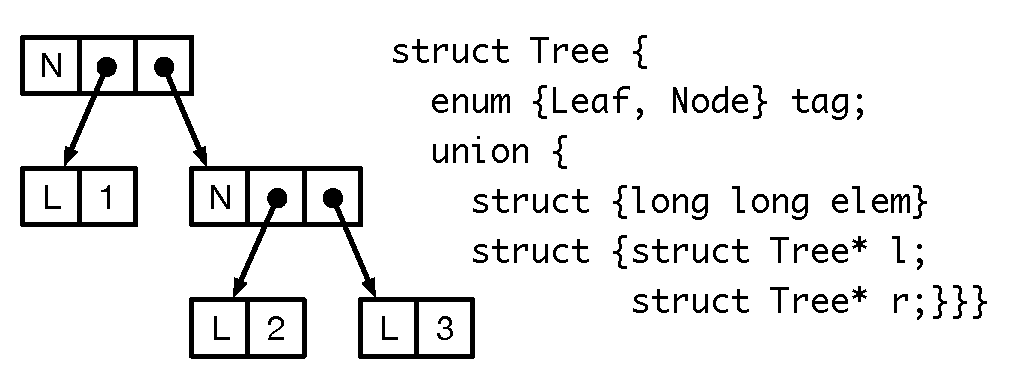
\includegraphics[scale=0.5]{figs/intro-tree-unpacked}
    \caption{Standard representation of a tree structure in C}
    \label{fig:intro-tree-unpacked}
  \end{subfigure}
  \begin{subfigure}[t]{\linewidth}
    \centering
    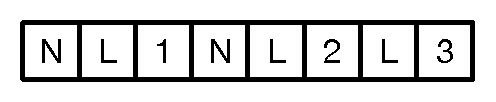
\includegraphics[scale=0.5]{figs/intro-tree-packed}
    \caption{Serialized version of the same tree}
    \label{fig:intro-tree-packed}    
  \end{subfigure}
  \caption{Standard and serialized representations of trees}
\end{figure}

% \begin{figure}
%% \begin{figure}
%% %\begin{wrapfigure}{r}{0.5\textwidth} 
%% \Red{PICTURE HERE:  possibly with wrapfig.}
% \begin{verbatim}
%  [N|.|.]          struct Tree {
%     /  \           enum { Leaf, Node } tag;
% [L 1]  [N|.|.]     union { 
%          /   \      struct { long long elem; };
%       [L 2] [L 3]   struct { struct Tree* l;
%                              struct Tree* r; }}}
% \end{verbatim}

%%   \caption{Traditional, pointer-based tree layout.}
%% \end{figure}
%\end{wrapfigure}
% \begin{verbatim}
%   [N L 1  N L 2  L 3 ]
% \end{verbatim}
% \end{figure}

Indeed, if we can compile programs to operate directly on this serialization, we
follow a precedent of using serialization formats jointly as in memory formats.
For example, Cap'N Proto \cite{capnproto} makes it ergonomic for C++ code to operate directly
on the Protobuf serialization format in memory.  Likewise ``data baking''
\cite{data-baking} is an established practice in video games---caching assets on
disk in a format that allows them to be \il{mmap}'d into memory and used
without further conversion.  As a general example of this capability, the
Glasgow Haskell Compiler (GHC) recently added the capability to store any closed
subgraph of the heap as a {\em Compact Normal Form} (CNF) \cite{cnf-icfp15}---a
contiguous memory region that is treated as a kind of ``super object'', never
traced by the GC and collected only when there are no pointers into any of the
sub-parts of the CNF.

The packed tree format above is precisely a dense encoding of a CNF---a
transitive closure of heap objects with no escaping pointers, in this case, no
pointers {\em at all}.  But unlike GHC's CNF support, which uses regular heap
objects, colocated together, the dense tree format {\em requires a complete
rearrangement of the compiled code that operates on the data}.

% Shall we acronymize it?
% DTF - dense tree form, or dense tree format
% PTF - packed tree form
% DTP - dense tree packing

In this paper, we take a first step towards compiler support for transparently
packing tree datatypes {\em without} changing the source program.  We make the
following contributions:

\newcommand{\calculus}{$\lambda^D_T$} % uh, Dense Tree?

\begin{itemize}
\item We use a small core language, \calculus{}, to formalize a transformation
  on programs with threes that creates an output program that operates only on
  pointers in the serialized representation.  This involves a small program
  synthesis step, and we show how the program synthesis and the selection of
  data structure shape go benefit from co-optimization.
  
\item We demonstrate that a prototype language implementation based on this
  transformation can compile a range of tree transforms to be several times
  faster than existing techniques~\cref{sec:eval-compiler}.
  
\item We show that the principle of packed-tree traversals works across a
  variety of language implementations, by benchmarking handwritten packed-tree
  programs~\cref{sec:eval-shootout}.
  
\item We show that not only do tree traversals become faster, but that their
  {\em potential parallel speedup}, increases as well \cref{sec:eval-parallel}.
\end{itemize}


% ================================================================================
% \section{Motivating Example}
\section{Background and Example}
% ================================================================================

While our main emphasis in this paper is on accelerating compiler passes, here
we continue with our simple example from the introduction: binary trees with
integer leaves.
In a language with algebraic datatypes,
% In a strongly typed functional language,
a recursive walk on
the tree would typically use pattern matching:

\ifcurly
% [language=python]
\begin{code}[language=c]
type Tree = Leaf(Int) | Node(Tree,Tree);

fun add1(t) {
  match(t) {
    Leaf(n):   return Leaf(n+1);
    Node(x,y): return Node(add1(x),add1(y));
  }}
\end{code}
\else
\begin{code}
 data Tree = Leaf Int | Node Tree Tree
  
 add1 t =
  case t of
    Leaf n   -> Leaf (n+1)
    Node x y -> Node (add1 x) (add1 y)
\end{code}
\fi

In fact, the small, first-order, purely functional language of tree traversals
we consider this paper is already a subset of most existing languages.
The above program is not substantially different in C, Haskell, ML, Scala,
Swift, Rust, etc.  Only the details of switching on sum types (tagged unions) differ.

The first problem for tree-walks such as this is memory management.  \il{add1}
can easy become a malloc or garbage collector benchmark.  For instance, the
following C code is over twice as slow as the same implementation in Java or a
good functional compiler:

\begin{code}[language=c]
  Tree* add1(Tree* t) {
    Tree* tout = (Tree*)malloc(sizeof(Tree));
    tout->tag = t->tag;
    if (t->tag == Leaf) {
      tout->elem = t->elem + 1;
    } else {
      tout->l = add1(t->l);
      tout->r = add1(t->r);
    }
    return tout;
  }
\end{code}

But even if we assume optimal layout, bump-pointer allocation, and {\em no
  header objects}---even if we go further and enable \il{__packed__} attribute
for our structs to save tag space---the performance of the above code is still
several times below what is achievable.  The main observation of this paper is
that bulk tree walks are efficient if done directly on pre-order serialization
of the tree, and that it is possible to automate the translation of recursive
functions, such as @add1@ above, into code that directly manipulates data
buffers containing serialized trees.

For our simple example, this buffer passing code isn't complicated:
%
\begin{code}[language=c]
char* add1(char* tin, char* tout) {
  if (*tin == Leaf) {
    *tout = Leaf;
    tin++; tout++;
    *(int*)tout = *(int*)tin;
    return (tin + sizeof(int));
  } else {
    *tout = Node;
    tin++; tout++;
    char* t2 = add1Tree(tin,tout);
    tout += (t2 - t);
    return add1Tree(t2,tout);
  }
}
\end{code}
%
Yet this approach cannot scale--it quickly becomes tedious and error prone.
Clearly, no one would use a technique like this for building a compiler!

The above program is similar to the output produced by the prototype compiler we
describe in this paper.  We refer to the input and output pointers as {\em
  cursors}, and one of the primary jobs of the compiler is automatic cursor
insertion.

%% \note{Yet, code performing raw manipulation of a pointer into a byte buffer
%%   containing a serialized tree is extremely error prone and tedious to write.
%%   It certainly is inappropriate for writing compilers, which contain reams and
%%   reams of tree-walking code.}

\subsection{Challenges and Limitations}

\note{Rightmost vs leftmost}


\ifcurly
\begin{code}[language=c]
fun left(t) {
  match(t) {
    Leaf(n):   return n;
    Node(x,_): return left(x);
  }}
fun right(t) {
  match(t) {
    Leaf(n):   return n;
    Node(_,y): return right(y);
  }}
\end{code}
\else
\begin{code}
 left t = case t of
            Leaf n   -> n
            Node x _ -> left x
 right t = case t of
             Leaf n   -> n
             Node _ y -> right y
\end{code}
\fi


\subsection{Related Work}

\rn{Milind, some of the related work was going to go up here?}

One line of closely related work focuses on managing data layout in trees and
other data structures to promote spatial
locality~\cite{Chilimbi1999,Chilimbi1999b,Truong1998,Lattner2005,Chilimbi1999a},
by modifying garbage collection to co-locate objects~\cite{Chilimbi1999a},
modifying memory allocators to proactively place objects with similar access
patterns together~\cite{Lattner2005,Chilimbi1999}, or to modify the internal
layout of objects to place hot fields near each other~\cite{Chilimbi1999b}.
These approaches attempt to ``pack'' data together, using various techniques,
into cache lines to improve spatial locality, and hence have some resemblance
to our packed representations, which gain some performance benefits from
packing tree data into a compact format that promotes spatial locality.

Perhaps the most closely related of these is Chilimbi et al.'s {\em cache
conscious structure layout}~\cite{Chilimbi1999}. They propose a
cache-conscious data placement scheme where, given a traversal function,
tree-structured data will be laid out in memory in a {\em clustered} manner:
nodes from small subtrees will be placed on single cache lines. By matching
the tree layout to a specified traversal order, spatial locality is improved
when the tree is traversed in that order. A key difference between our packed
representation and Chilimbi et al.'s work is that this work focused on object
layout, without changing the internal {\em representation} of the objects.
Leaving the object representation of tree nodes the same allows code that
manipulates the objects to remain the same, but incurs costs: there is no
opportunity to reduce the space or instruction overhead incurred by pointers
linking nodes in the tree (see Figure~\ref{fig:intro-fig}), as exploiting that
opportunity requires code transformation. Most of the aforementioned spatial
locality work makes the same tradeoff.

One exception is Chilimbi et al.'s work on {\em automatic structure
splitting}~\cite{Chilimbi1999b}, where objects are transformed into split
representations, allowing hot fields from multiple objects to be co-located on
a single cache line while those objects' cold fields are placed elsewhere.
Because this layout optimization changes the internal representation of the
object, Chilimbi et al. develop a compiler pass that automatically transforms
code to work with the split representation. The transformations for structure
splitting concern how to access object fields, and hence, unlike our work, do
not require deeper transformations to remove the pointer dereferences inherent
in traversing linked data structures.


% ================================================================================
\section{The \treelang{} Language}
% ================================================================================

\note{Informal overview of language}

To demonstrate the compilation technique we are presenting, we present
$\treelang{}$, a typed programming language that is simple enough to
present briefly in a paper, and featureful enough to express some
interesting programs, such as common compiler passes.

Programs consist of a series of data type declarations and function
declarations. Similar to most functional programming languages,
programmers may define \emph{algebraic data types}, and dispatch on
them with a \texttt{match} language form (called \texttt{case} or
\texttt{switch} in some languages).
%% For example, a data type for peano
%% numbers would have two cases: zero and successor.

\note{We already gave an example of a program in TreeLang earlier...
  probably only need one, unless we're doing something different here}

%% \begin{code}[language=haskell]
%% type Nat = Zero | Suc(Nat);
%% \end{code}

%% For simplicity, $\treelang{}$ is a first-order language, so all
%% functions are defined at the top level.

%% \begin{code}[language=haskell]
%% fun trav(x) {
%%   match(x) {
%%     Zero: return 0;
%%     Suc(n): return 1 + trav(n);
%% }}
%% \end{code}

In addition to algebraic data types and various numerical types, $\treelang{}$ supports
general purpose persistent dictionaries, which are useful for implementing compiler
passes in a functional style.

\note{Show an example of using a dictionary? Or just give the types?}

\note{Describe the Racket front-end and how it works.}

% ================================================================================
\section{Formal Language}
% ================================================================================


\note{The calculus, plus the core lowering transforms in figures.}

We present two languages: L1, a simple purely functional, first-order programming
language with sum and product types; and L2, an imperative programming language
with mutable arrays and pointer arithmetic, as well as a type-and-effect system.

\subsection{L1: Source language}

%% \note{Do we have a problem if we just stick to the way sums and products are usually presented?
%%   Or do we need recursive types? Also, binary sums and products might make the switch form
%%   in L2 less interesting.}

\note{This is horribly outdated and needs to be rewritten.}

\begin{figure}
  \begin{displaymath}
    \begin{aligned}
      \keywd{prog} \gramdef & \keywdr{d} \keywdr{f} \keywd{e} \\
      \keywd{d} \gramdef & \keywd{type} \keywd{D} (\keywd{K} \keywdr{t})^{*} \\
      \keywd{f} \gramdef & \keywd{fun} \keywd{F} ( \keywdr{V} ) { \keywdr{e} } \\
      \keywd{t} \gramdef & \keywd{Int} \gramor \keywd{Sym} \gramor \keywd{Bool} \\
      \gramor & \keywd{Vector} \keywdr{t} \gramor \keywd{SymDict} \keywd{t} \\
      \keywd{e} \gramdef & \keywd{V} \gramor \keywd{n} \gramor \keywd{f} \keywdr{e} \\
      \gramor & \keywd{vector} \keywdr{e} \gramor \keywd{vector-ref} \keywd{e} \keywd{n} \\
      \gramor & \keywd{F} \keywdr{e} \gramor \keywd{case} \keywd{e} (K \keywdr{V})^{*} \keywd{e} \\
      \gramor & \keywd{let} (\keywd{V} \keywd{e})^{*} \keywd{e} \\
      \gramor & \keywd{if} \keywd{e} \keywd{e} \keywd{e} \gramor \keywd{primapp} \\
      \gramor & \keywd{error} \keywd{str} \gramor \keywd{time} \keywd{e}  
    \end{aligned}
  \end{displaymath}
  \caption{Grammar for source language}
\end{figure}

\subsection{L2: Target language}

\begin{figure}
\begin{displaymath}
  \begin{aligned}
    \keywd{x} \gramdef & \keywd{n} \gramor \keywd{v} \\
    \keywd{t} \gramdef & \keywd{int} \gramor \keywd{cursor} \gramor \keywd{t} \rightarrow \keywd{t} \gramor \keywd{t} * \keywd{t} \\
    \keywd{e} \gramdef & \keywd{x} \gramor \keywd{x} \keywd{p} \keywd{x} \gramor \keywd{v} \keywd{x} \\
    \gramor & \keywd{(x,x)} \gramor \# 1 \keywd{x} \gramor \# 2 \keywd{x} \\
    \gramor & \keywd{let} \keywd{(v,t,e)} \keywd{e} \\
    \gramor & \keywd{ifeq} \keywd{(x,x)} \keywd{e} \keywd{e} \\
    \gramor & \keywd{switch} \keywd{x} \keywdr{(n,v,e)} \\
    \gramor & \keywd{newbuff} \keywd{n} \\
    \gramor & \keywd{writetag} \keywd{v} \keywd{n} \\
    \gramor & \keywd{writeint} \keywd{v} \keywd{x} \\
    \gramor & \keywd{readtag} \keywd{v} \\
    \gramor & \keywd{readint} \keywd{v} 
  \end{aligned}
\end{displaymath}
\caption{Grammar for target language}
\end{figure}

% ================================================================================
% \section{A tree-packing compiler}
\section{Compilation Algorithms}
% ================================================================================

\note{The central issue in compiling \treelang, is deriving runtime witnesses of
  the {\em end} of values in memory.  If we recursively unpack adjacent fields
  without storing a pointer to the later fields, we must rediscover those
  downstream fields as a side effect of traversing their upstream ones.}



\subsection{Inferring effects}
% ----------------------------------------

% \newcommand{\arr}[3]{\ensuremath{{#1} \xrightarrow{\overrightarrow{#2}} {#3}}}
% \newcommand{\arr}[3]{\ensuremath{{#1} \xrightarrow{trav({#2})} {#3}}}
\newcommand{\arr}[3]{\ensuremath{{#1} \xrightarrow{#2} {#3}}}
% $\xrightarrow[world]{hello}$

We denote a function with traversal effects as \arr{A}{\alpha}{B}, meaning a
function that traverses the value located at $\alpha$ during its execution.


\begin{figure}
\begin{verbatim}
    Top
  Fixed a   Fixed b   ....
  Fresh a   Fresh b   ....
    Bottom
\end{verbatim}
  \caption{The lattice for abstract location analysis.}
  \label{fig:lattice}
\end{figure}


\subsection{Copy and traversal insertion}
% ----------------------------------------


\note{During analysis, we generated all the information we need not only to {\em
    label} traversal effects, but to recognize where they are needed, but
  missing.}

\note{With the inter-procedural traversal types settled, we reprocess the and
  perform the same location analysis, but wherever we are missing a witness of a
  field stored within a packed buffer, we perform a program synthesis to
  generate a recursive call that meets that constraint.}

\note{We insert calls to only two functions---copy and insert---whose
  definitions the compiler generates in a subsequent pass.}

\note{Even still, there's a search space of potential places to insert code.  We
  follow a simple heuristic of introducing traversals in as large a scope as
  possible, e.g. just under a case expression that binds the field variables.}
%% directly at the point of missing constraints.  This may introduce the same
%%   traversal multiple times, for example within different branches of an If

\subsection{Routing end-of-value witnesses}
% ----------------------------------------


\subsection{Reordering to discover witnesses}
% ----------------------------------------

\note{At this point in the compilation process, ``witnesses'' have been inserted,
  and code has been generated to consume them. The program is not necessarily valid,
  however, because the places in the code where witnesses are consumed are not
  guaranteed to be within the scope of the binders that introduced the witness.}

\note{Briefly explain why we generate code weirdly like this.}

\note{Due to the fact that our programs have few effects (can we say they're
  purely functional?), and that our programs are in A-normal form (each sub-expression
  is bound to a name), we can represent a program as a graph where each bound name
  is a node and its edges are the bindings it depends on. A correct reordering of
  a program is a topological sort of this graph.}



\subsection{Output cursor insertion}
% ----------------------------------------

\note{Locally dilated representation of packed values.}

\newcommand{\END}[1]{\ensuremath{\overline{#1}}}

\note{Several ways to encode these:}

\begin{code}
  (Tree@$_a$@,Tree@$_b$@)

  ((Cur@$_a$@,Cur@$_{\END{a}}$@),(Cur@$_b$@,Cur@$_{\END{b}}$@))

  ((Cur@$_a$@,Cur@$_b$@),(Cur@$_{\END{a}}$@,Cur@$_{\END{b}}$@))
\end{code}


\subsection{Code generation}
% ----------------------------------------

\note{Programs are compiled to C code.}

\note{The compiler walks through the program to accumulate all
  anonymous product (tuple) types, and emits C struct declarations for
  each.}

\note{In the intermediate language, cursors are returned along with
  the ordinary return value during any operation on a buffer---for
  example, reading an int from a cursor returns the int and a new
  cursor. A simple implementation strategy for this would be a
  function that returns a struct of int and cursor, but we have found
  that even when such a function is marked for inlining it is slower
  than directly inlining the code and avoiding the returned struct.
  So, when translating this into C code, we generate a series of C
  declarations, with each variable only assigned once. We attempt to
  avoid the creation of structs whenever possible, preferring to
  inline operations that return tuples and to unzip tuples into
  ordinary variables.}
  
\note{C code is linked with a simple ``run time system'' (a C file with
  some helper procedures and benchmark harnesses).}


% ================================================================================
\subsection{Discussion}
% ================================================================================

\note{Purity is important to reordering for witness search.}

\note{Our interpreter depends on this fact by modeling cursors {\em as lists}.}


% ================================================================================
\section{Implementation}
% ================================================================================

\note{Current prototype implementation, status}



% ================================================================================
\section{Evaluation}
% ================================================================================

We evaluate the performance of our approach in four ways. First, we
demonstrate via small microbenchmarks that packed data representation
provides significant performance wins across a variety of
languages---including languages with good performance on pointer-based
traversals---and that our compiler produces code competetive with any
existing system. Second, we build several standard compiler passes
operating on Racket's intermediate representation, and show
substantial speedup operating on inputs gathered from existing Racket
programs. Third, we build a type checker for a small language, and
benchmark it on large synthetic inputs, demonstrating significant
speedup for a more complex and data-heavy workload. Fourth, we
implement a point-correlation benchmark using a kd-tree, again showing
major performance benefits for packed representations. Additionally,
we \note{something something parallel}

All benchmarks were conducted on a \dots.

\subsection{Microbenchmarks}
% ----------------------------------------

Our first benchmarks return to the example from section 2,
manipulating simple binary trees. We implement 3 operations:
constructing a tree, incrementing the values in a tree, and summing
the elements of a tree. To understand the performance of packed data
representations, we implemented these three operations in multiple
ways across a variety of languages: with pointer-based trees in
Racket, Chez Scheme, MLton, GHC Haskell, and C (using both \texttt{malloc} as well
as a fast bump-pointer allocator). We also implemented packed versions
using handwritten C code similar to that of section 2, as well as a
packed version in Racket. Finally, we implemented the benchmark in
\treelang{}, and executed it using both the simple Racket backend and
the optimizing backend that is the focus of this paper.

The results show a clear win for packed representations, in some cases
with 100x speedup over pointer-based representations in
garbage-collected languages. Further, our compiler-generated code is
competetive with handwritten C for packed data.

%\note{A ``language shootout'' of add1-tree benchmarks.}


\subsection{Compiler passes on realistic inputs}
% --------------------------------------------

\note{Racket core AST benchmarks}


\subsection{Typechecking benchmark}
% --------------------------------------------

\note{type check the simply-typed $\lambda$ calculus in \treelang{}}

\subsection{Point correlation}
% --------------------------------------------
Point correlation  is a well-known algorithm that is used in data mining\cite{capnproto},
given a point p in a k-dimensional space, a radius r, and a set of points in the space,
point correlation computes the number of nodes that are within a distance r from the point p.
One efficient way of doing that is to use kd-trees  to store the set of points in the space\cite{capnproto}. 

A kd-tree is a binary space partitioning tree that in its simplest form  splits the space at each internal node into two spaces
around a split axes in one of the space dimensions, the left subtree stores the points on the left of the split access
and the right subtree sotres the points on the right of the split access, the split axes alternates between the dimensions of
the space at each level of the tree, when the number of the points in the subtree is one a 
leaf node that stores one point of in the space is constructed .

In a naive implementation point correlation need to be executed at each leaf node for each input point, however kd-trees 
allow  it to  prune early by storing at each internal node the boundaries within which all descendent points lies,
and use that information to skip a subtree if the given point is far enough from the boundaries.

We evaluate two versions of the point correlation traversal,intOut and treeOut; intOut version
produces an integer as the output of the traversal while  tree out version  produces a tree
that have the same data of the input tree with the some counters in the leaf nodes that 
correlates with the input point updated.Unlike  the rest of the benchmarks that are  evaluated in this paper,
 the intOut version does not need to traverse the whole tree due to the early trucation, this requires
the packed version to store the address of the right child for each internal node.Tree out version on the other hand 
does not need that additional field, although the computation might  truncate at some points during the traversal, 
the whole tree always need to be traversed to copy the data from the input tree to the output tree, 
and the right child address is always available.

The traversals are implemented in c++, and for each of the two variants, three different implementation are compared ; 
a pointer based implementation that uses the standard allocation techniques, a pointer based implementation that uses bump allocation, 
and a packed implementation as described in section .... 

The intOut version requires 63\% less amount of memory to represent the tree , and the outTree requires 55\% less memory ,when
the size of the tree is large the saving is large ,table .. shows that amount of memory saving for different tree sizes,for treeOut 
yet it also enhances the performance.

Figure .. shows the runtime speedups of over the standerd pointer based implementations for the packed and bump-allocation versions, 
although it might 

 
\subsection{Parallelism opportunity study}
% --------------------------------------------

\note{Report preliminary parallel microbenchmark results, showing the potential
  for future work here.}




% ================================================================================
\section{Future work}
% ================================================================================

\note{Data type factoring, storing leaves in a separate, dense, aligned vector.
This enables (1) vectorization of numeric operations, and (2) separating
out pointers that the GC must traverse.  This can prove essential for an
open-world implementation in a managed language.}


\note{A large space of parallelism design choices.}

\note{}


%% % ================================================================================
%% \appendix
%% \section{Appendix Title}
%% % ================================================================================

%% This is the text of the appendix, if you need one.

%% \acks

%% Acknowledgments, if needed.

% \bibliographystyle{abbrvnat}
\bibliographystyle{abbrv}

% If you can't commit to the submodule right this second, just copy
% this file to ./refs.bib :
\bibliography{bibs/refs}

% The bibliography should be embedded for final submission.
%% \begin{thebibliography}{}
%% \softraggedright
%% \bibitem[Smith et~al.(2009)Smith, Jones]{smith02}
%% P. Q. Smith, and X. Y. Jones. ...reference text...
%% \end{thebibliography}


\end{document}


